This chapter examines the findings and critiques various steps of this thesis. The first two sections compare the models' performances both quantitatively and qualitatively. The third section elucidates the limitations and possible improvements and proposes potential directions for research on children's drawings.

\section{Quantitative Performance Analysis}

FT Aug Mini Replica, the Mini-Replica fine-tuned using the examples of drawing-artwork pairs, is the best model for retrieving artworks similar to a drawing. The model finds the relevant artwork in the first 400 results with a 88\% probability. Although the likelihood of finding the relevant artwork falls to 54\% in the first 20 results, it is still nearly two times more probable than using a CNN model trained for image classification. FT Aug, the model fine-tuned on the pre-trained ResNeXt-101, is the second-best model. FT Aug's performance is similar to that of Mini-Replica - the fine-tuned CNN to retrieve duplicate artwork photographs and fine-tuning Mini-Replica enhances the performance. FT No-Aug Clus-Replica does not retrieve visually relevant results, albeit showing the third-best performance.

The examples of drawings shown in this thesis portray their variousness; some drawings are pencil sketches of artworks that are photographs, some drawings used colored pencils to re-create the paintings, or in some cases, the artworks were in grayscale, and the drawing was in color. These differences make it challenging to create correspondences between the drawing and artwork only with one example. At the same time, there could be an unidentified drawing in the current dataset or a new drawing in the future that uses different techniques and materials than the artwork. Experimentation shows that the style augmentation step made it possible to overcome this hurdle.

The mean average precision comprises precision and recall. It becomes a vital measure indicating how well the model detects the correct artwork for a drawing, and it increases from close to 17\% to little more than 37\% in the top three models. 

Unlike the MAP and Recall, the trend in the mean positions of the artworks is different. The models that do not use style augmented drawings for training have relatively lower mean positions than those that use them. The mean position averages the rank of the relevant artwork across all possible artworks, and it is skewed if there is more than one possible match, and one appears early while the other is ranked low. This contradiction between the mean position and other measures results from overfitting the models with limited examples (No-Aug cases). In some examples of drawings, it is possible to have more than one similar artwork. Table \ref{tab:test-mmp} contains a new Minimum Mean Position (MMP) measure that computes the mean position using one lowest rank per drawing on the test dataset (Excluding the No-Aug models). The best-performing models remain the same with a slight change in their order. FT Aug has the lowest MMP, followed by FT Aug Mini-Replica and FT Aug Clus-Replica. Earlier measures suggest that the Mini-Replica achieves a performance similar to that of a fine-tuned pre-trained model (FT Aug) without task-specific fine-tuning. Nonetheless, the MMP depicts that the FT Aug ranks the artworks better than the Mini-Replica except for a few cases discussed in the next section.

\begin{table}[ht]
 \centering
    \begin{tabular}{c||c}
        \hline
        Model & {MMP} \\ \hline \hline
        \textit{Baseline} & 1491.63 ± 360.31 \\
        \textit{FT Aug} & \textbf{231.48 ± 134.63} \\
        \textit{Mini-Replica} & 416.90 ± 263.74 \\
        \textit{FT Aug Mini-Replica} & {285.21 ± 160.47} \\
        \textit{Clus-Replica} & 536.80 ± 214.68 \\
        \textit{FT Aug Clus-Replica} & 429.87 ± 214.67 \\
    \end{tabular}
    \caption{Minumum Mean position of drawings in Test data}
    \label{tab:test-mmp}
\end{table}

All these experiments use a minimal set of examples and achieve satisfactory performances. Nevertheless, the lower standard deviation in the Replica models is a striking difference between the FT Aug and the Replica variants. The large datasets used in training could explain the low variation in the metrics of the Mini-Replica, Clus-Replica, and their fine-tuned versions. The performance of Replica models is better than the pre-trained model because the knowledge of identifying duplicate paintings is close and related problem to the drawing-artwork problem.

\section{Qualitative Performance Analysis}

Evaluation metrics convey a model's performance and do not capture the results' quality. This section discusses the ranking grade by comparing six models: Baseline, FT Aug, Mini-Replica, FT Aug Mini-Replica, Clus-Replica, and FT Aug Clus-Replica. The best variant of each model during the 11-fold validation was used to create the feature vectors and compare the images. Each comparison image contains three parts where the drawing is at the top left, and expected similar artwork is at the bottom left of the image. Lastly, the top 10 retrievals using the six models mentioned above are on the right side of the image, along with the rank of the expected artwork. The rank is helpful, especially if the expected artwork does not appear in the top 10 results.


\subsection{Closely Imitated Drawings}

\afterpage{
    \clearpage
    % \thispagestyle{empty}
    \begin{landscape}
    \centering
    \begin{figure}
     \centering
     \begin{subfigure}[b]{0.55\textwidth}
         \centering
         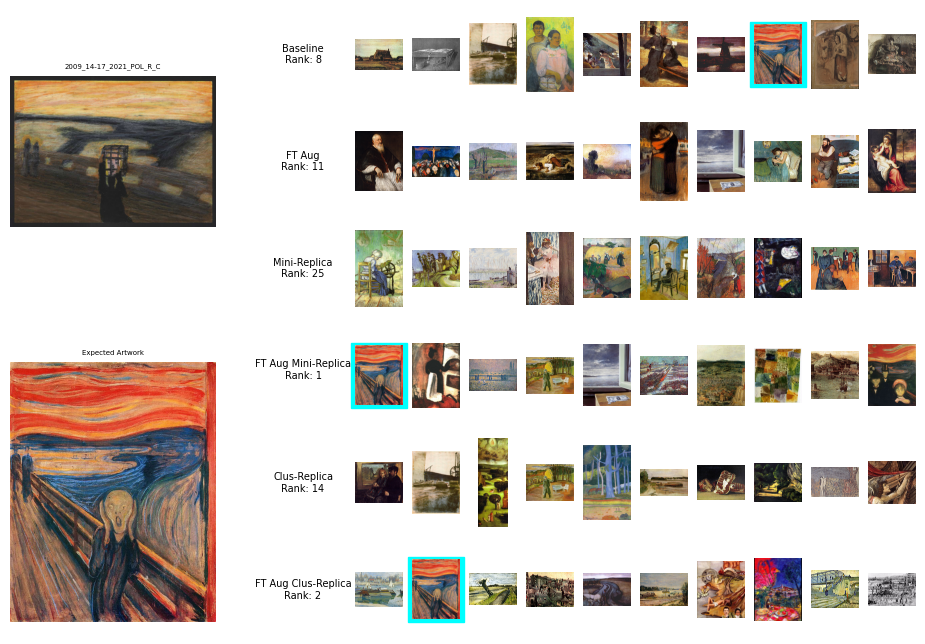
\includegraphics[width=1.01\textwidth]{images/qualitative_analysis/2009_14-17_2021_POL_R_C.png}
         \caption{Drawing: \texttt{2009\_14-17\_2021\_POL\_R\_C} part of training set}
         \label{fig:2009_14-17_2021_POL_R_C}
     \end{subfigure}
     \hfil
     \begin{subfigure}[b]{0.55\textwidth}
         \centering
         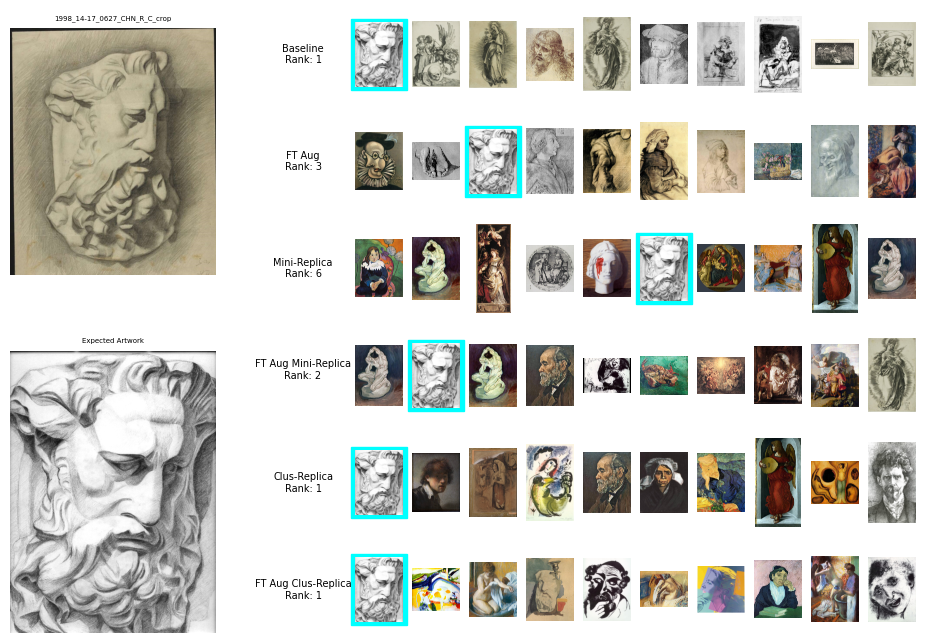
\includegraphics[width=1.01\textwidth]{images/qualitative_analysis/1998_14-17_0627_CHN_R_C_crop.png}
         \caption{Drawing: \texttt{1998\_14-17\_0627\_CHN\_R\_C} part of training set}
         \label{fig:1998_14-17_0627_CHN_R_C_crop}
     \end{subfigure}
     \hfil
     \begin{subfigure}[b]{0.55\textwidth}
         \centering
         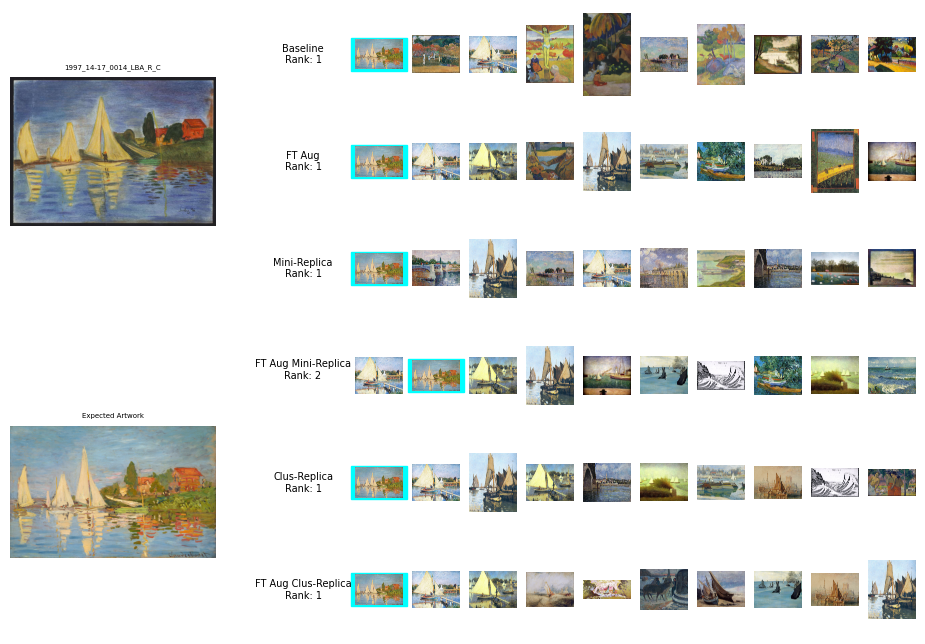
\includegraphics[width=1.01\textwidth]{images/qualitative_analysis/1997_14-17_0014_LBA_R_C.png}
         \caption{Drawing: \texttt{1997\_14-17\_0014\_LBA\_R\_C} part of test set}
         \label{fig:1997_14-17_0014_LBA_R_C}
     \end{subfigure}
     \hfil
     \begin{subfigure}[b]{0.55\textwidth}
         \centering
         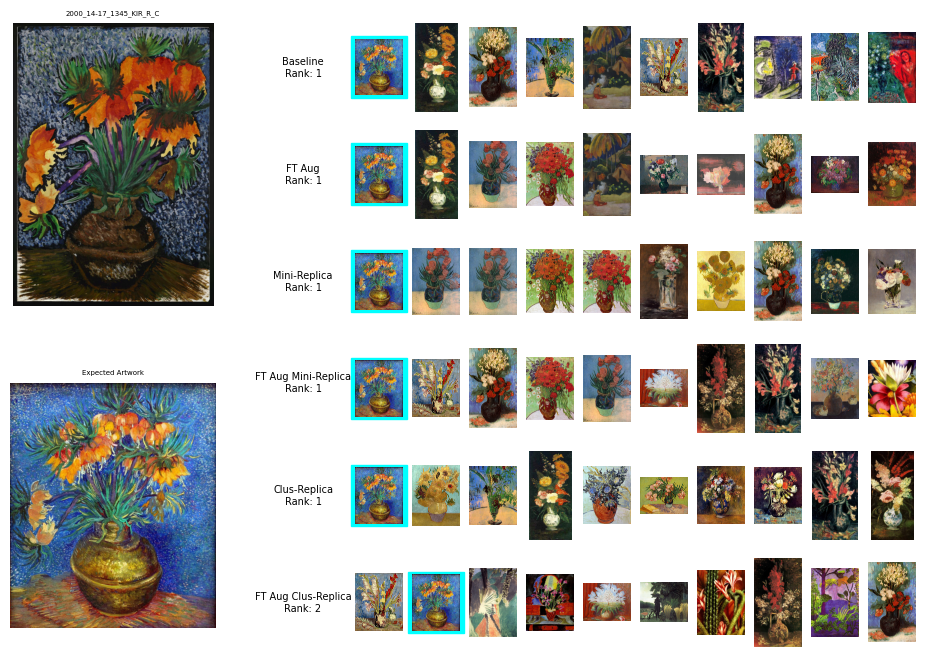
\includegraphics[width=1.01\textwidth]{images/qualitative_analysis/2000_14-17_1345_KIR_R_C.png}
         \caption{Drawing: \texttt{2000\_14-17\_1345\_KIR\_R\_C} part of validation set}
         \label{fig:2000_14-17_1345_KIR_R_C}
     \end{subfigure}
        \caption{Top 10 retrievals of drawings close to original artwork}
        \label{fig:baseline-best}
\end{figure}

    \end{landscape}
    \clearpage
}

Many computer vision problems use CNN architectures developed for ImageNet image classification as a starting point as the layers have already learned to detect features such as the color and shape of objects. Although the overall performance of these models is poor in drawing-artwork retrieval, they identify the relevant artwork when the drawing is close to the compared artwork. Figure \ref{fig:baseline-best} shows such examples; in each of them, the drawing replicates the artwork very closely. Even when there is a slight color change, the baseline model ranks the appropriate artwork at the top. 

\subsection{Domain and Technique Constrainted Retrieval}

Another problem with the baseline model is its inability to retrieve artworks produced using a different technique than the drawing. Figure \ref{fig:technique-limitation} shows some examples. The Replica variants retrieve these examples even before fine-tuning, and fine-tuning ranks them better. In the case of Figures \ref{fig:2009_14-17_1234_DEU_R_C} and \ref{fig:1998_14-17_0293_LBA_R_C}, the baseline model only retrieves artworks made using pencil sketches, while the relevant artwork is not a pencil sketch. The consequence of fine-tuning is visible in the results, making the artworks appear in the top positions with FT Aug and FT Aug Mini-Replica, overcoming the difficulty of recognizing the artwork produced using a different technique.

The artwork's material distinguishes it from a sketch, photograph, computer-generated image, or painting. Figure \ref{fig:domain-limitation} compares the retrieval of artworks in examples where the method and material of the drawings are in contrast to the artwork. Similar to the previous discussion, the Mini-Replica and FT Aug models can overcome the domain limitations.

All in all, the Replica variants do not suffer from the difference in techniques between the artwork and drawings. However, their performance is slightly affected when the domain is different. Nevertheless, fine-tuning the baseline or the Replica variants helps confound it.

\afterpage{
    \clearpage
    % \thispagestyle{empty}
    \begin{landscape}
    \centering
    \begin{figure}
     \centering
     \begin{subfigure}[b]{0.55\textwidth}
         \centering
         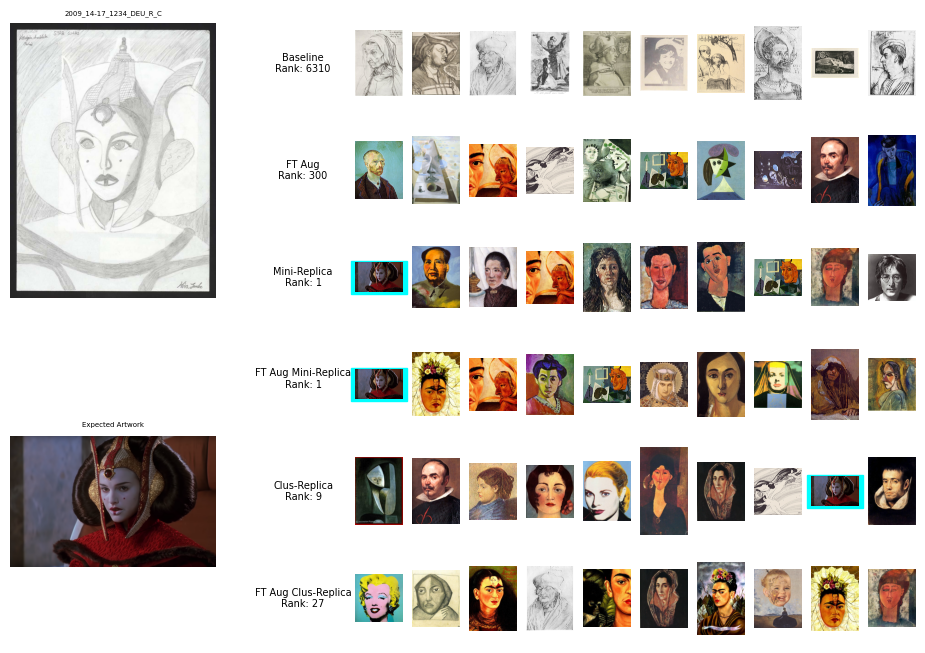
\includegraphics[width=1.01\textwidth]{images/qualitative_analysis/2009_14-17_1234_DEU_R_C.png}
         \caption{Drawing: \texttt{2009\_14-17\_1234\_DEU\_R\_C} part of training set}
         \label{fig:2009_14-17_1234_DEU_R_C}
     \end{subfigure}
     \hfil
     \begin{subfigure}[b]{0.55\textwidth}
         \centering
         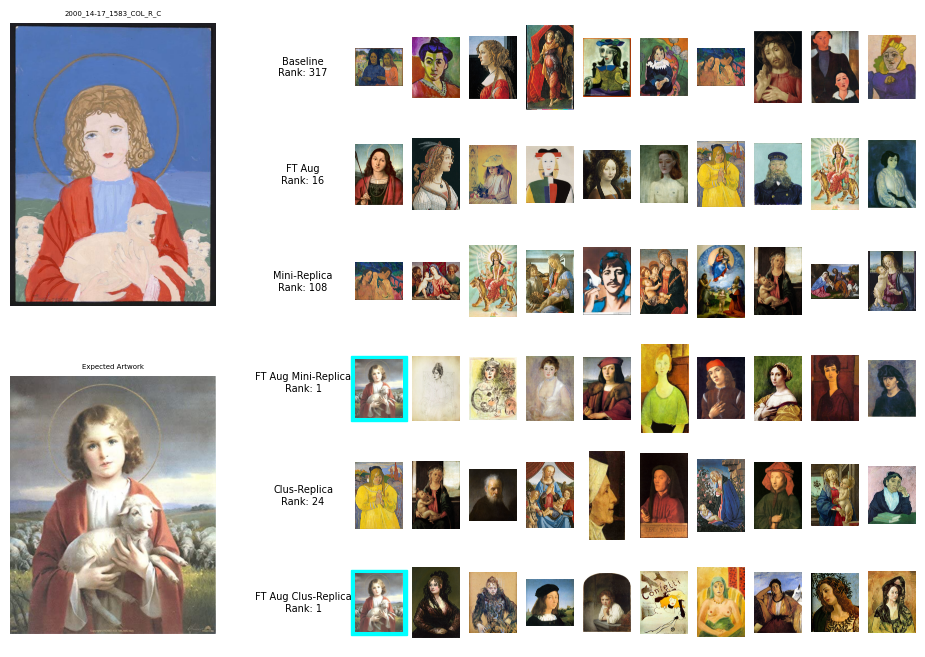
\includegraphics[width=1.01\textwidth]{images/qualitative_analysis/2000_14-17_1583_COL_R_C.png}
         \caption{Drawing: \texttt{2000\_14-17\_1583\_COL\_R\_C} part of training set}
         \label{fig:2000_14-17_1583_COL_R_C}
     \end{subfigure}
     \hfil
     \begin{subfigure}[b]{0.55\textwidth}
         \centering
         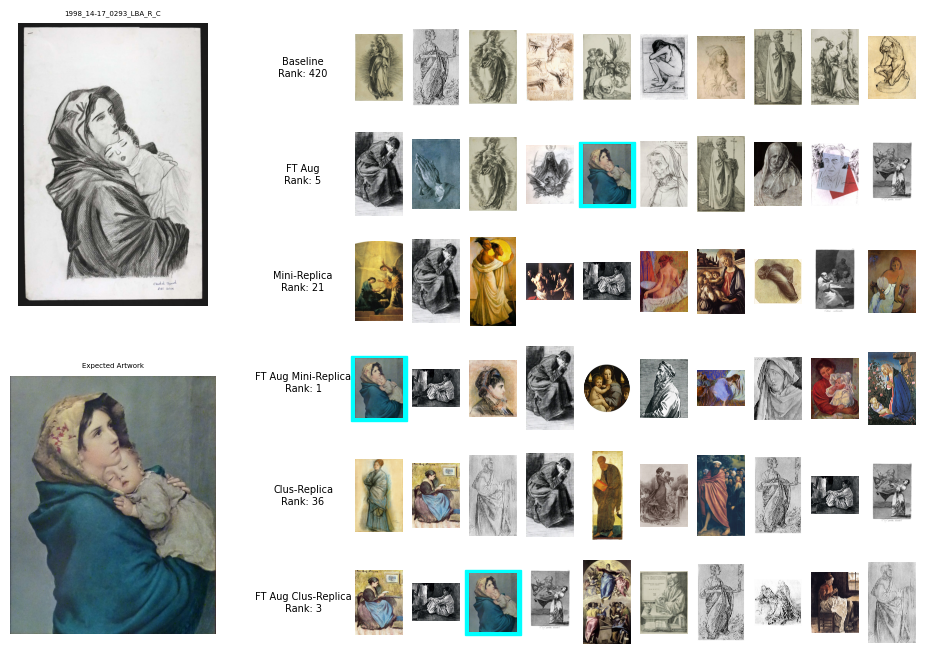
\includegraphics[width=1.01\textwidth]{images/qualitative_analysis/1998_14-17_0293_LBA_R_C.png}
         \caption{Drawing: \texttt{1998\_14-17\_0293\_LBA\_R\_C} part of training set}
         \label{fig:1998_14-17_0293_LBA_R_C}
     \end{subfigure}
     \hfil
     \begin{subfigure}[b]{0.55\textwidth}
         \centering
         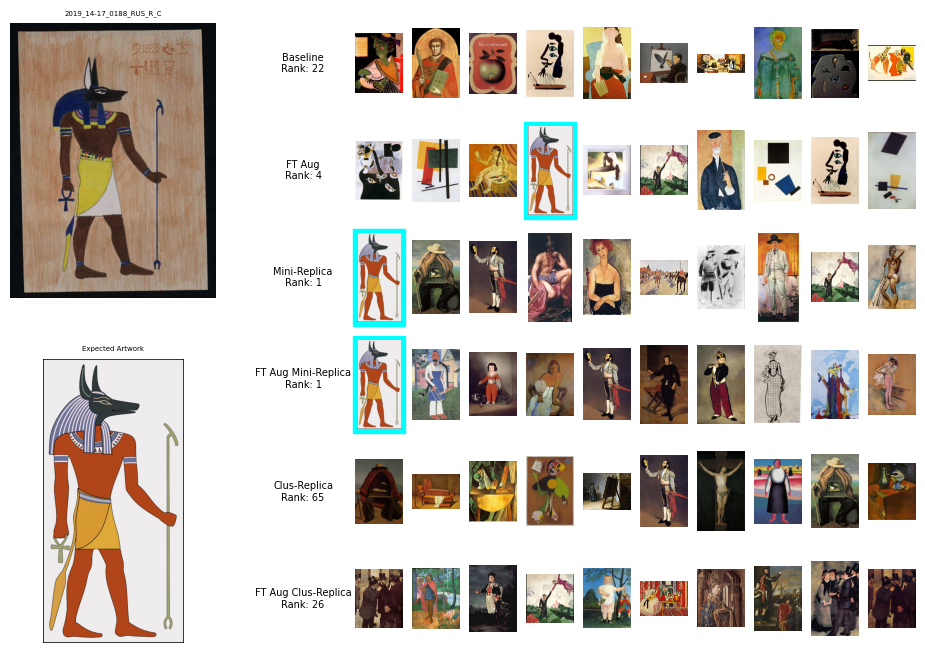
\includegraphics[width=1.01\textwidth]{images/qualitative_analysis/2019_14-17_0188_RUS_R_C.png}
         \caption{Drawing: \texttt{2019\_14-17\_0188\_RUS\_R\_C} part of validation set}
         \label{fig:2019_14-17_0188_RUS_R_C}
     \end{subfigure}
        \caption{Top 10 retrievals of drawings using a different drawing technique than the original artwork}
        \label{fig:technique-limitation}
\end{figure}

    \end{landscape}
    \clearpage
}


\afterpage{
    \clearpage
    % \thispagestyle{empty}
    \begin{landscape}
    \centering
    \begin{figure}
     \centering
     \begin{subfigure}[b]{0.55\textwidth}
         \centering
         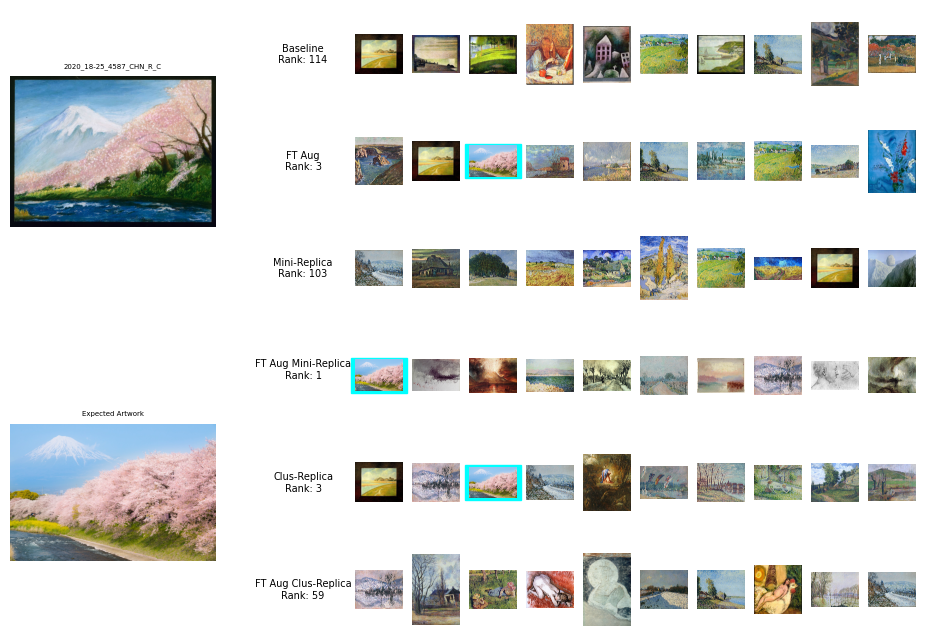
\includegraphics[width=1.01\textwidth]{images/qualitative_analysis/2020_18-25_4587_CHN_R_C.png}
         \caption{Drawing: \texttt{2020\_18-25\_4587\_CHN\_R\_C} part of training set}
         \label{fig:2020_18-25_4587_CHN_R_C}
     \end{subfigure}
     \hfil
     \begin{subfigure}[b]{0.55\textwidth}
         \centering
         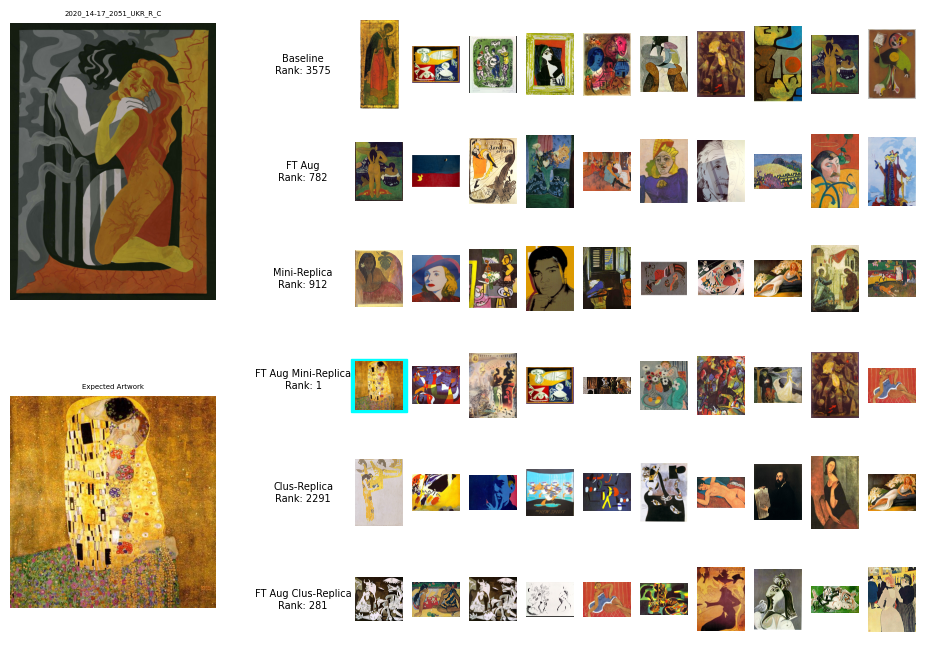
\includegraphics[width=1.01\textwidth]{images/qualitative_analysis/2020_14-17_2051_UKR_R_C.png}
         \caption{Drawing: \texttt{2020\_14-17\_2051\_UKR\_R\_C} part of training set}
         \label{fig:2020_14-17_2051_UKR_R_C}
     \end{subfigure}
     \hfil
     \begin{subfigure}[b]{0.55\textwidth}
         \centering
         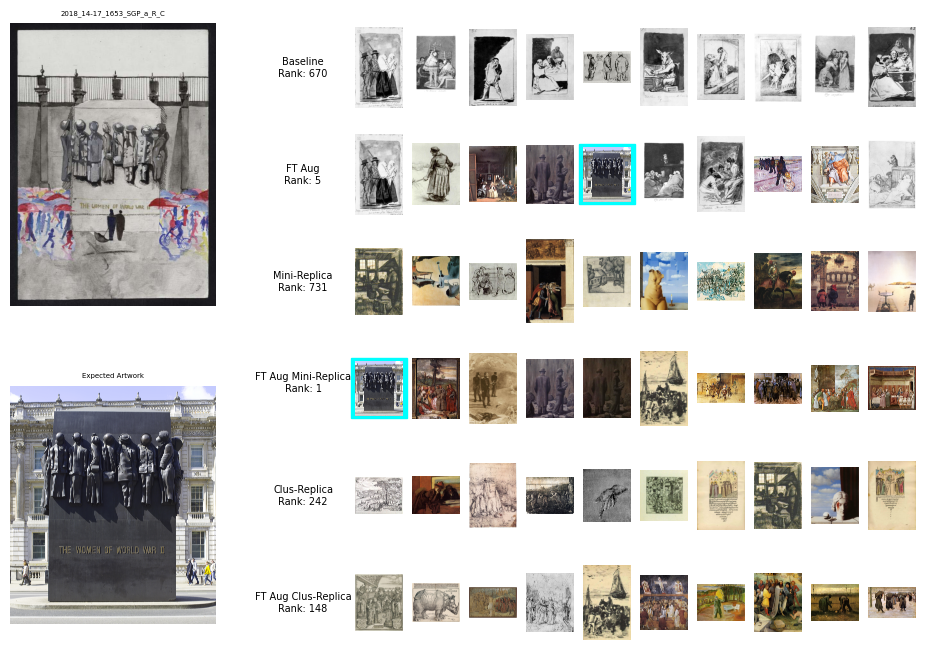
\includegraphics[width=1.01\textwidth]{images/qualitative_analysis/2018_14-17_1653_SGP_a_R_C.png}
         \caption{Drawing: \texttt{2018\_14-17\_1653\_SGP\_a\_R\_C} part of training set}
         \label{fig:2018_14-17_1653_SGP_a_R_C}
     \end{subfigure}
     \hfil
     \begin{subfigure}[b]{0.55\textwidth}
         \centering
         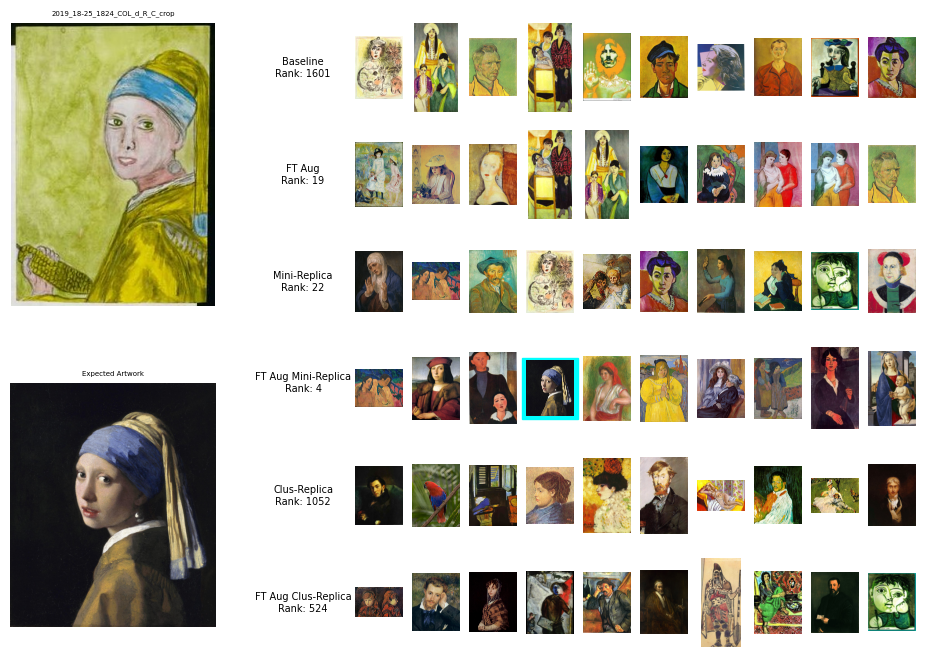
\includegraphics[width=1.01\textwidth]{images/qualitative_analysis/2019_18-25_1824_COL_d_R_C_crop.png}
         \caption{Drawing: \texttt{2019\_18-25\_1824\_COL\_d\_R\_C} part of validation set}
         \label{fig:2019_18-25_1824_COL_d_R_C_crop}
     \end{subfigure}
        \caption{Top 10 retrievals of drawings in a different domain than the original artwork}
        \label{fig:domain-limitation}
\end{figure}

    \end{landscape}
    \clearpage
}


\subsection{Differences between the Replica variants}

Qualitative analysis of the results clearly shows that the results of the Clus-Replica are inferior to that of the Mini-Replica and FT Aug in many cases. Notwithstanding the evaluation metrics, the retrievals of Clus-Replica and its fine-tune are not up to the mark. Inspection of the results reveals that FT Aug and Mini-Replica models learn the object localization and the semantic meaning of the drawing while Clus-Replica focuses on global average information (shape, color). The retrieval examples in Figure \ref{fig:replica-differences} shows these differences.

Although Mini-Replica and the Clus-Replica models start with the same base, train using metric learning, and have heavily overlapping training data, their objectives differ. The former model aims to find photos sharing a pattern, while the latter tries to cluster all such artwork photographs. The loss function in metric learning translates these differences in the objectives to training. The Mini-Replica model, whose training is similar to the drawing-artwork problem, moves the artwork similar to a drawing close to it than the dissimilar ones. In addition to Mini-Replica, Clus-Replica also ensures that images in a cluster are within a specified limit. Thus, optimizing one cluster of works impacts the other clusters and increases the probability of outlier images overflowing into other clusters and producing semantically undesirable results in this project.


\afterpage{
    \clearpage
    % \thispagestyle{empty}
    \begin{landscape}
    \centering
    \begin{figure}
     \centering
     \begin{subfigure}[b]{0.55\textwidth}
         \centering
         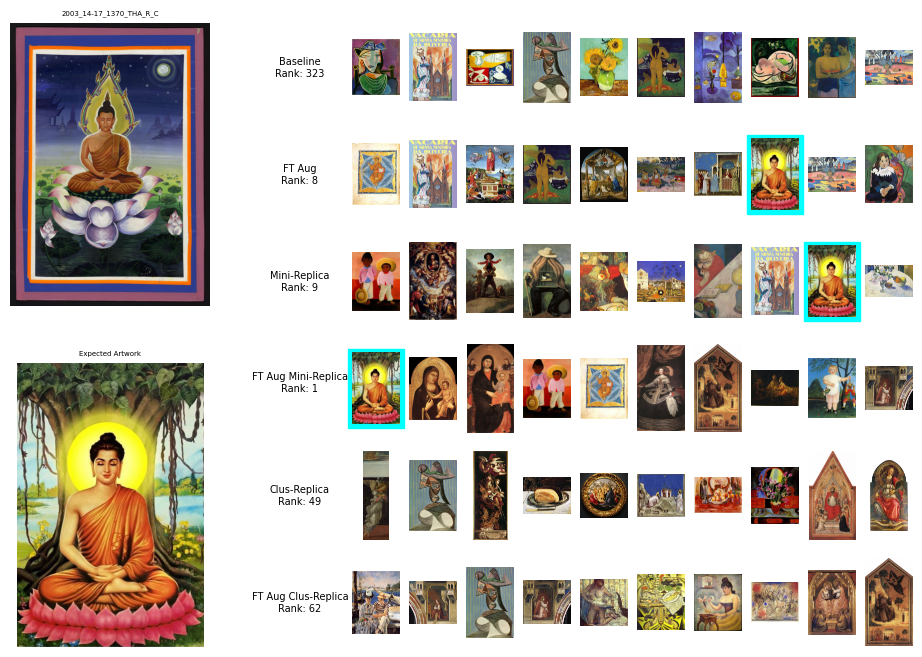
\includegraphics[width=1.01\textwidth]{images/qualitative_analysis/2003_14-17_1370_THA_R_C.png}
         \caption{Drawing: \texttt{2003\_14-17\_1370\_THA\_R\_C} part of training set}
         \label{fig:2003_14-17_1370_THA_R_C}
     \end{subfigure}
     \hfil
     \begin{subfigure}[b]{0.55\textwidth}
         \centering
         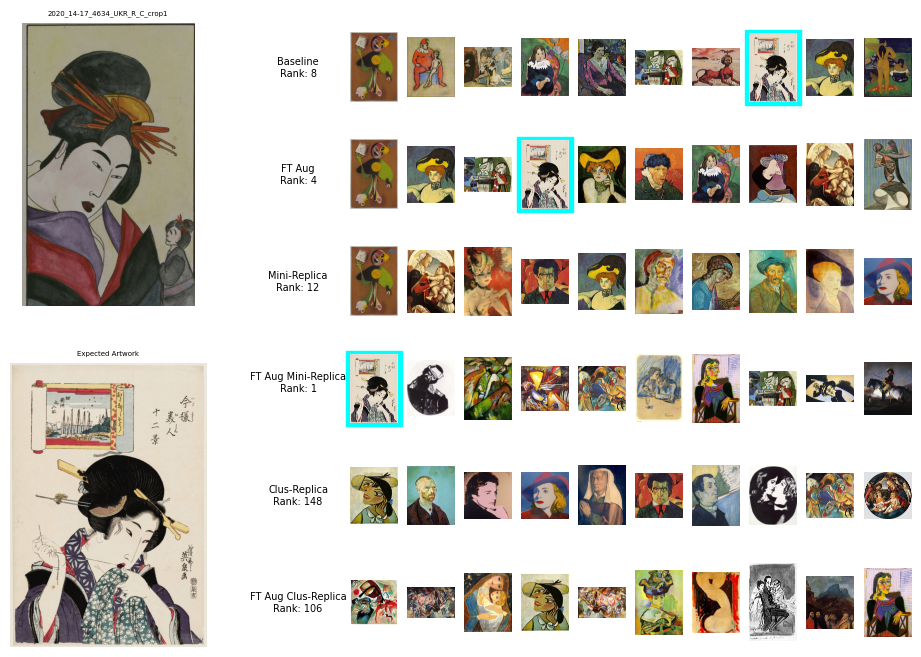
\includegraphics[width=1.01\textwidth]{images/qualitative_analysis/2020_14-17_4634_UKR_R_C_crop1.png}
         \caption{Drawing: \texttt{2020\_14-17\_4634\_UKR\_R\_C} part of training set}
         \label{fig:2020_14-17_4634_UKR_R_C_crop1}
     \end{subfigure}
     \hfil
     \begin{subfigure}[b]{0.55\textwidth}
         \centering
         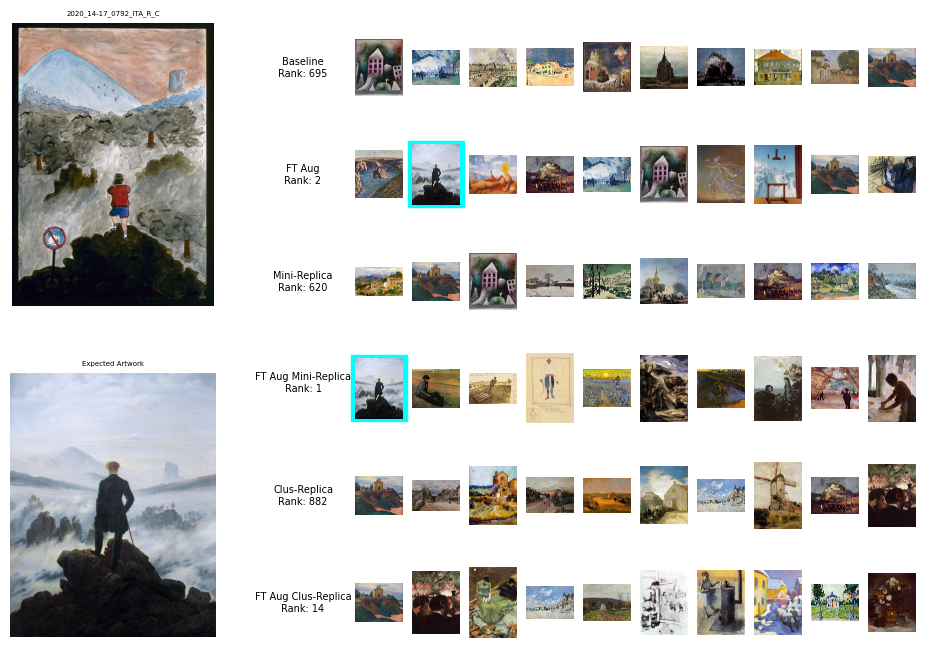
\includegraphics[width=1.01\textwidth]{images/qualitative_analysis/2020_14-17_0792_ITA_R_C.png}
         \caption{Drawing: \texttt{2020\_14-17\_0792\_ITA\_R\_C} part of training set}
         \label{fig:2020_14-17_0792_ITA_R_C}
     \end{subfigure}
     \hfil
     \begin{subfigure}[b]{0.55\textwidth}
         \centering
         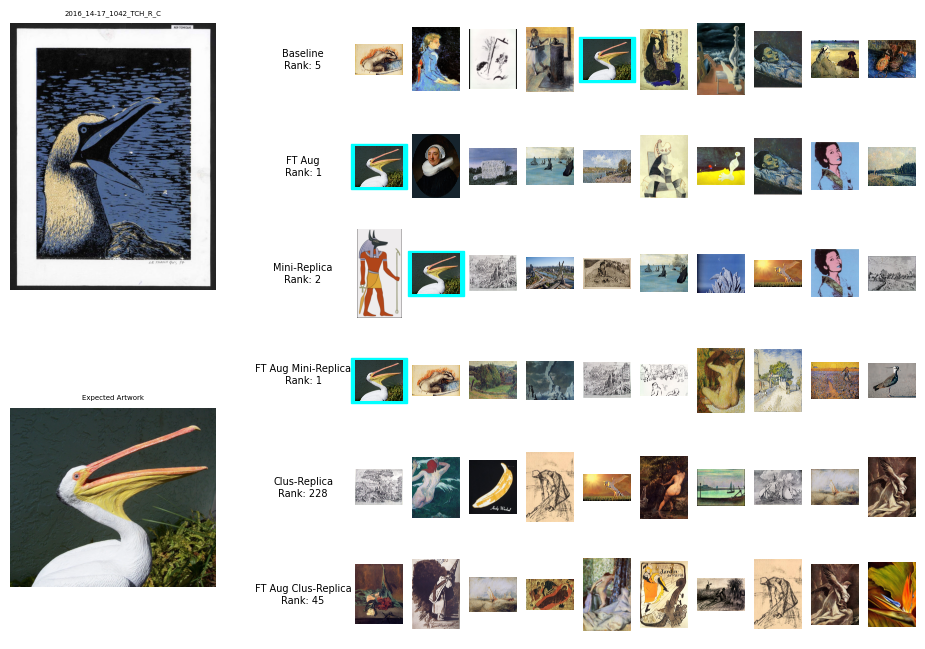
\includegraphics[width=1.01\textwidth]{images/qualitative_analysis/2016_14-17_1042_TCH_R_C.png}
         \caption{Drawing: \texttt{2016\_14-17\_1042\_TCH\_R\_C} part of test set}
         \label{fig:2016_14-17_1042_TCH_R_C}
     \end{subfigure}
        \caption{Examples depicting Clus-Replica's poor quality retrievals}
        \label{fig:replica-differences}
\end{figure}

    \end{landscape}
    \clearpage
}

\subsection{Failure modes}

The examples in the previous sections show drawings whose artwork appears in the top results. There are three categories of failures, and Figure \ref{fig:breakdown} showcases them. The first mistake is when a single element dominates the drawing. In Figures \ref{fig:2019_18-25_2298_MEX_R_C} and \ref{fig:2013_14-17_1011_POL_R_C}, the retrieved artworks have predominantly white and black backgrounds, owing to the color of the paper and cardboard used to make those drawings. Figure \ref{fig:2000_14-17_0443_UKR_R_C} shows an example of the second category of mistakes where fine-tuned models push the artwork backward in the ranks. All these examples are in validation or test set, and they did not directly affect the parameters of the models. The last category is those with weak visual similarities. Although the relevant artwork does not appear in the first ten results in Figure \ref{fig:2010_MS_0981_FRA_R_C}, it moves closer to artworks as reflected in the ranks.

\afterpage{
    \clearpage
    % \thispagestyle{empty}
    \begin{landscape}
    \centering
    \begin{figure}
     \centering
     \begin{subfigure}[b]{0.55\textwidth}
         \centering
         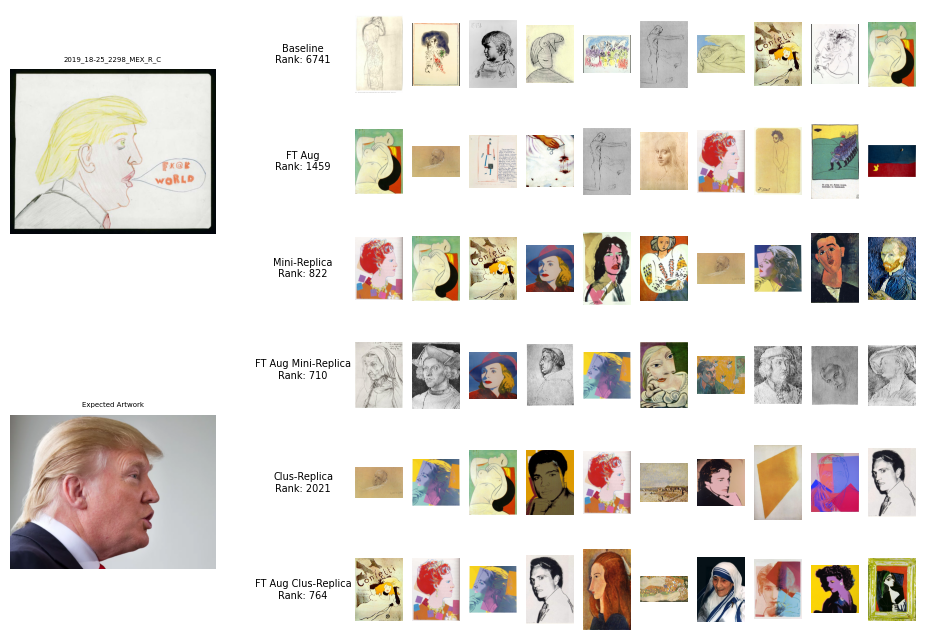
\includegraphics[width=1.01\textwidth]{images/qualitative_analysis/2019_18-25_2298_MEX_R_C.png}
         \caption{Drawing: \texttt{2019\_18-25\_2298\_MEX\_R\_C} part of validation set}
         \label{fig:2019_18-25_2298_MEX_R_C}
     \end{subfigure}
     \hfil
     \begin{subfigure}[b]{0.55\textwidth}
         \centering
         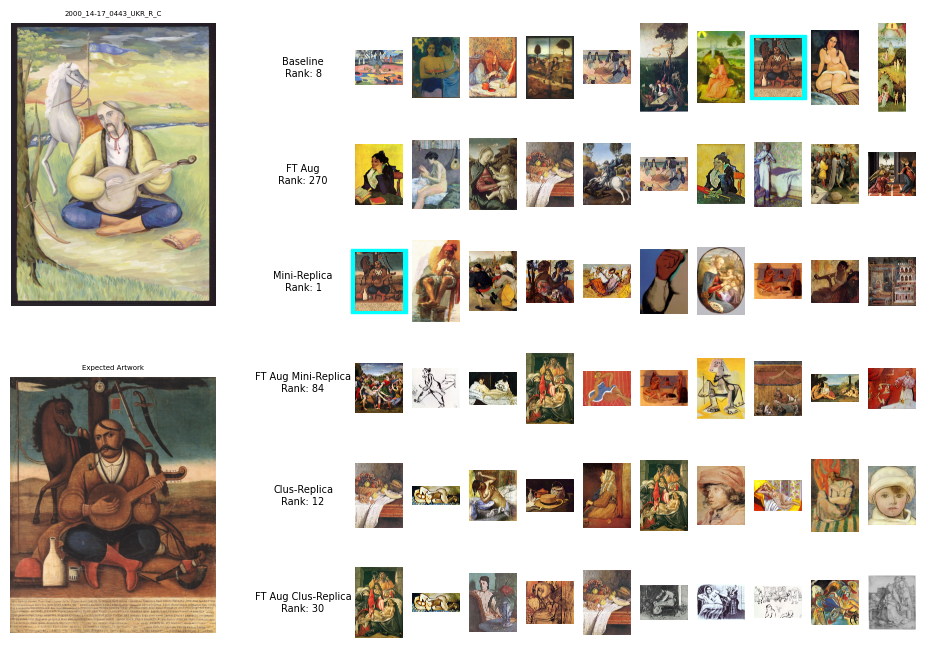
\includegraphics[width=1.01\textwidth]{images/qualitative_analysis/2000_14-17_0443_UKR_R_C.png}
         \caption{Drawing: \texttt{2000\_14-17\_0443\_UKR\_R\_C} part of validation set}
         \label{fig:2000_14-17_0443_UKR_R_C}
     \end{subfigure}
     \hfil
     \begin{subfigure}[b]{0.55\textwidth}
         \centering
         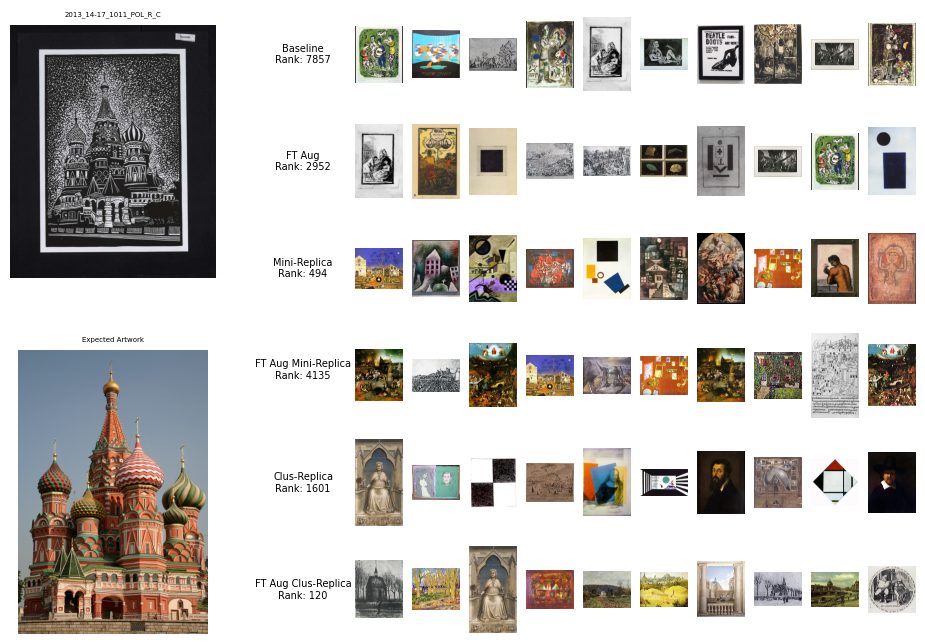
\includegraphics[width=1.01\textwidth]{images/qualitative_analysis/2013_14-17_1011_POL_R_C.png}
         \caption{Drawing: \texttt{2013\_14-17\_1011\_POL\_R\_C} part of test set}
         \label{fig:2013_14-17_1011_POL_R_C}
     \end{subfigure}
     \hfil
     \begin{subfigure}[b]{0.55\textwidth}
         \centering
         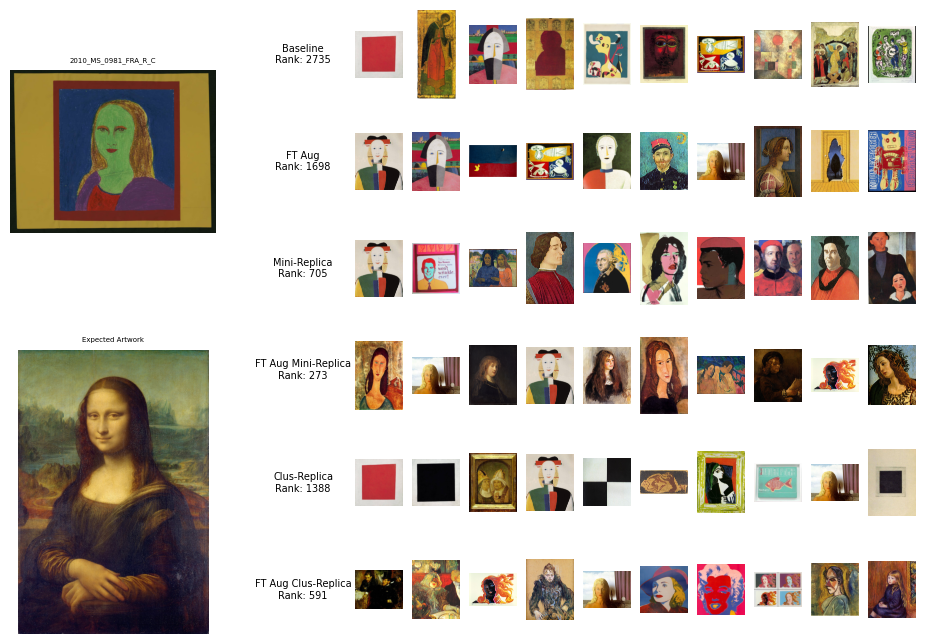
\includegraphics[width=1.01\textwidth]{images/qualitative_analysis/2010_MS_0981_FRA_R_C.png}
         \caption{Drawing: \texttt{2010\_MS\_0981\_FRA\_R\_C} part of test set}
         \label{fig:2010_MS_0981_FRA_R_C}
     \end{subfigure}
        \caption{Breakdown examples}
        \label{fig:breakdown}
\end{figure}

    \end{landscape}
    \clearpage
}

\section{Limitations and Future Work}

This project suffers from three drawbacks. Firstly, the choice of the artworks dataset. The artworks and the artists primarily fall in the Europe region without sufficient representation of works from the rest of the world, especially from the Eastern nations where a sizable number of drawings originate. While using the artworks from the digitized collections of museums of WikiArt would partially solve this problem, it increases the computational complexity involved in the online mining of the triplets. Additionally, many drawings refer to other pop culture objects, which are not necessarily paintings or drawings by famous artists. Supplementing the paintings dataset with popular cultural objects such as posters, shots in movies, portraits of celebrities, and others would unearth more drawing-artwork pairs.

Secondly, it was only possible to annotate a hundred examples of valid drawing-artworks during the project term. Increasing the number of examples does not constantly improve the models' performance. Nonetheless, having more annotated data helps to understand whether the relatively high variation in the metrics is inherent to the data or is only due to the low number of samples. The models developed during the project comes in handy in this aspect as they can aid in identifying new drawing-artwork pairs, subject to the availability of the relevant artwork in the comparison dataset.

Experimentation on the image's resolution was not part of the project, as the choice of 280 resulted from the trade-off between memory and computation time. Also, a comparison with sketch retrieval models is missing, particularly in using existing Sketch-Based Image Retrieval (SBIR) models as the starting point and fine-tuning them for the specific task. Thus, a future investigation of the image size and comparison with SBIR models would provide more cognizance.

Future work could expand the drawings dataset to include the drawing of 6-13-year-olds to the current 14-25-year-olds. In terms of the model architecture, an investigation to use more recent computer vision deep learning models is possible, significantly as the number of annotated examples increases. Another interesting exploration avenue is creating a retrieval system based on the similarity in the style or semantic meaning. 

Lastly, the current system helps identify the drawings similar to other drawings in the drawings dataset. Reading the identical drawings with their metadata and temporality shall characterize the propagation of ideas across years. The previous suggestions are mainly technical directions, but this research also has a social aspect. The artwork ranking model, along with metadata about the young artists' country and that of the relevant artwork, provides insights into the cross-cultural influences of the famous artists and their work. In addition, Section \ref{chap:3:sec:research-dir} lists a set of possible explorations on the drawings dataset itself.